Pour l'authentification du client au niveau de sa banque, nous avons opté pour une implémentation
externe d'un service d'authentification. De ce fait, nous séparons bien le développement de
l'application de la banque et son authentification.
L'authentification du client est une fonctionnalité primordiale pour le fonctionnement de l'ACS.

\section{Keycloak}

\begin{figure}[H]
    \centering
    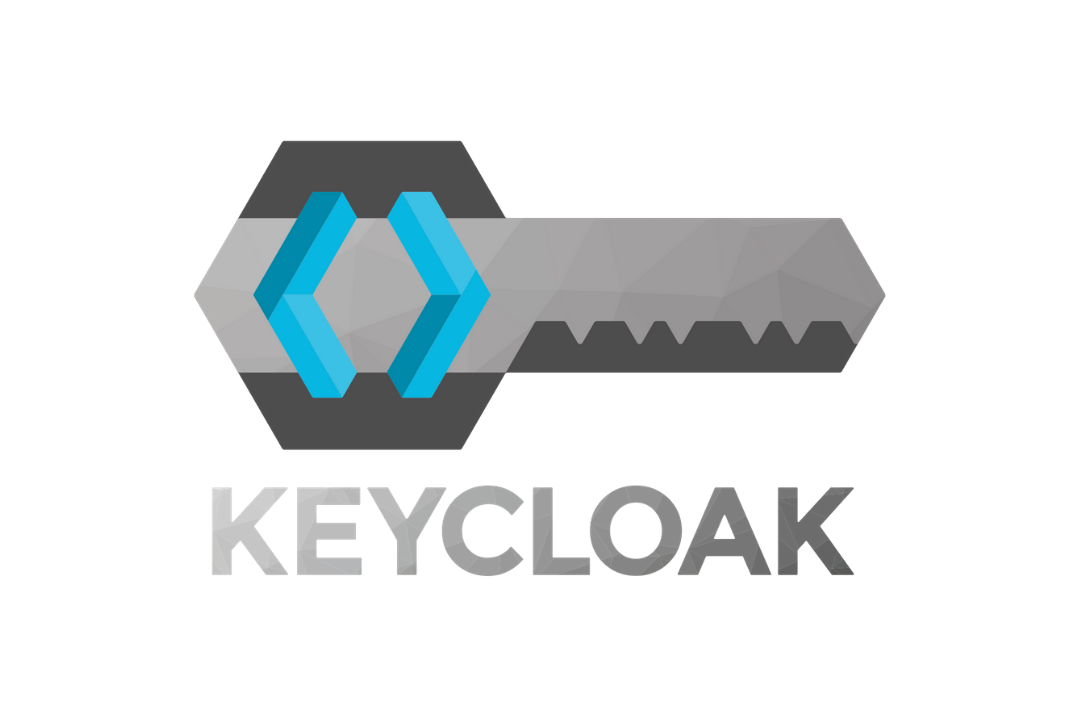
\includegraphics[scale=.1]{./img/Keycloak.png}
    \caption{Icône du logiciel Keycloak}
    \label{fig:keycloak_logo}
\end{figure}

Keycloak est un software d'authentification open-source
possédant une grande communauté. Ce software est
utilisé pour l'authentification de plusieurs entreprises à
travers le monde, ce qui nous rapproche d'une
infrastructure réelle. Nous l'avons choisi pour:

\begin{itemize}
    \item Séparer la partie fonctionnelle de l'ACS et
    l'authentification du client
    \item Créer une plateforme d'authentification la plus
    fidèle possible à la réalité
    \item Apprendre de nouvelles technologies
\end{itemize}

Keycloak possède plusieurs fonctionnalités appréciables à la création du projet. Notamment le
déploiement via Kubernetes ou Docker.

\subsubsection{Single-Sign On (SSO)}

Keycloak implémente la fonction de SSO : le client n'a besoin de s'authentifier qu'une seule fois et
sera automatiquement connecté si le token créé à la première connexion est toujours valide.

\subsubsection{Connexion à des base de données existantes}

Keycloak peut se connecter à une base de données relationnelle existante, mais aussi un serveur
Active Directory ou LDAP. Cela permet de créer plusieurs instances de keycloak connecté à la même
base de données.

\begin{figure}[H]
    \centering
    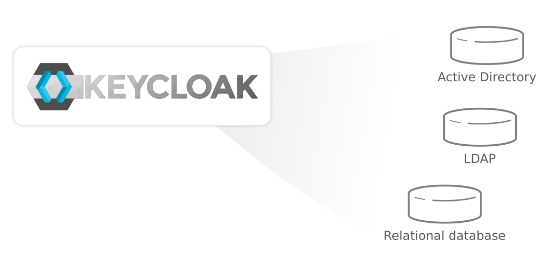
\includegraphics[width=\textwidth]{./img/Keycloak-Existant-Data.png}
    \caption{Différentes sources de données peuvent être configurées pour Keycloak}
    \label{fig:keycloak_data_source}
\end{figure}

\subsubsection{Identity Providers}

Keycloak prend le rôle d'Identity Provider via les protocoles OpenID Connect (OIDC), OAuth 2.0 ou
SAML 2.0. Cela nous permet de nous connecter en utilisant des librairies implémentant ces deux
protocoles. Pour l'application web de la banque, faite en React, nous avons utilisé la librairie react-
oidc d'AXA (le groupe d'assurance).

Mais ce n'est pas tout. Grâce à cette implémentation, nous pouvons aussi nous identifier par des
Identity Provider existant, tel que Google, Github, Facebook, \dots

\begin{figure}[H]
    \centering
    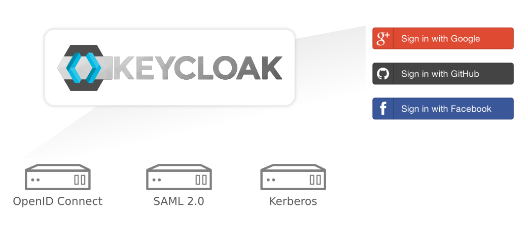
\includegraphics[width=\textwidth]{./img/Keycloak-Identity-Provider.png}
    \caption{Keycloak et ses différents IDP}
    \label{fig:keycloak_idp}
\end{figure}

\subsection{Fonctionnement}

\subsubsection{Authentification}

Le principe de keycloak est, comme énoncé dans l'introduction, de séparer la partie d'authentification
de la partie fonctionnement de l'ACS. Pour se faire, le client va essayer de se connecter à l'ACS, mais
sera redirigé vers Keycloak. Si l'authentification est réussie, le client pourra accéder à l'ACS. Si le client
essaie de se reconnecter, Keycloak va vérifier si le token généré est toujours valide et si c'est le cas, va
directement rediriger le client à l'ACS (fonctionnement du SSO).

Le formulaire de connexion sera détaillé plus tard, dans la partie Authentication Flow.

\begin{figure}[H]
    \centering
    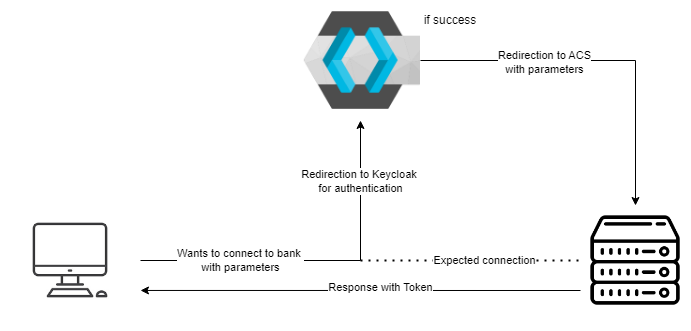
\includegraphics[width=\textwidth]{./img/Keycloak-Authentication-Process.png}
    \caption{Processus d'authentification}
    \label{fig:keycloak_auth}
\end{figure}

\subsubsection{Realms}

Keycloak intègre la notion de royaumes, ou realms qui implémente chacun leur client de connexion,
leurs utilisateurs, leurs serveurs SMTP, ... Ces realms permettent par exemple de créer une
infrastructure par site pour une entreprise possédants plusieurs sites.

Prenons l'exemple de l'entreprise John Cockerill. En implémentant un realm pour le site de Seraing et
un autre pour le site de Loncin, les administrateurs du site de Seraing ne peuvent pas interagir sur le
site de Loncin.

Bien évidemment, il y a un realm master, permettant d'interagir en tant qu'administrateur. Ce realm
est unique et est le seul permettant d'interagir sur les autres realms.

\begin{figure}[H]
    \centering
    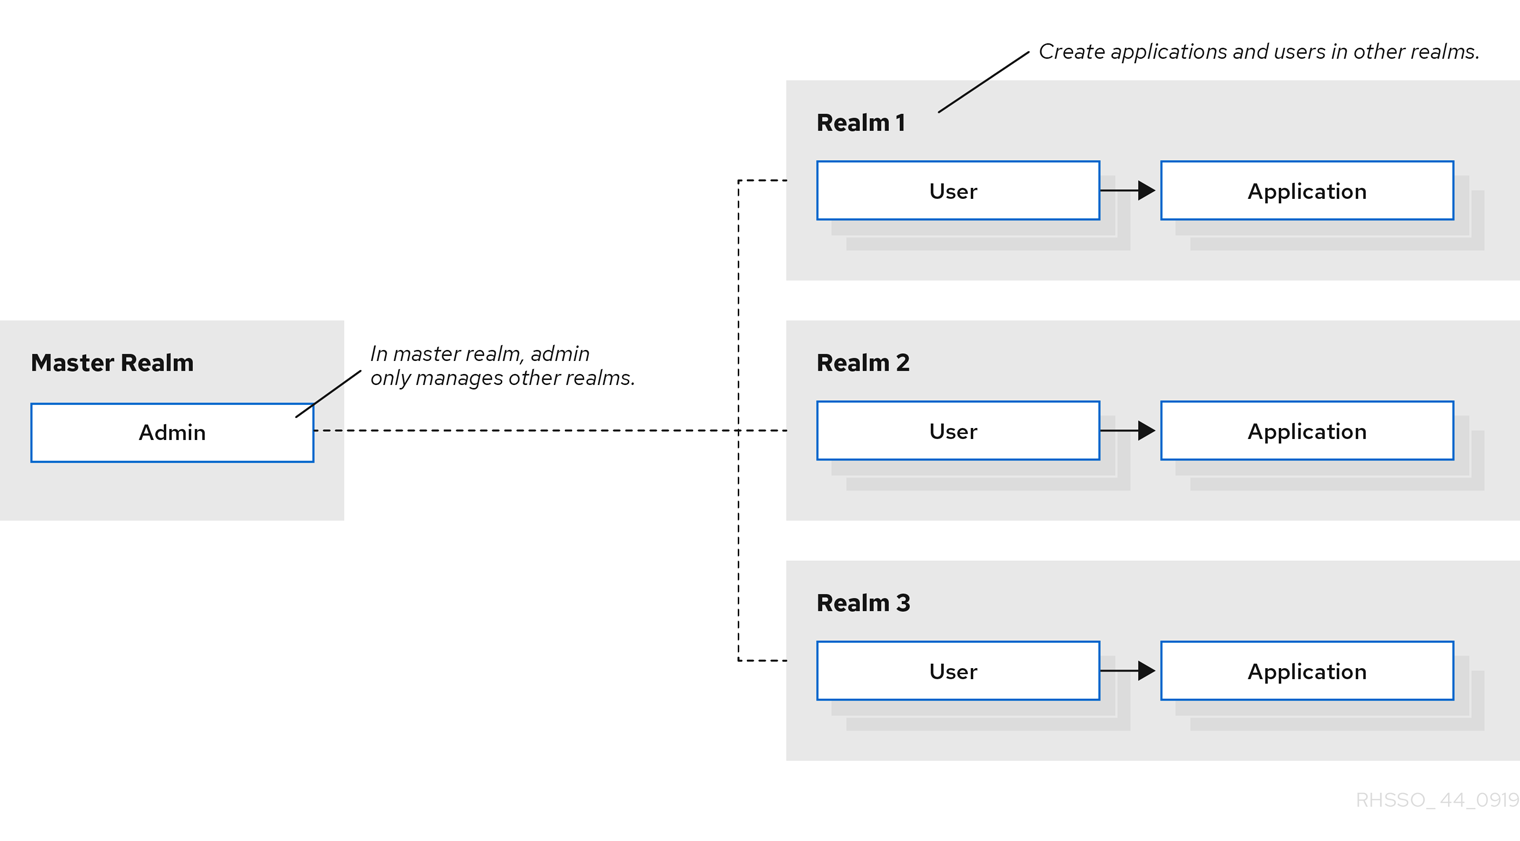
\includegraphics[width=\textwidth]{./img/Keycloak-realm.png}
    \caption{Les Realms ou "Royaumes" de Keycloak}
    \label{fig:keycloak_realms}
\end{figure}

\subsubsection{Clients}

Les clients représentent les moyens de connexion disponible sur le realm. Ces clients possèdent
plusieurs paramètres :

\paragraph{Root URL:} l'url qui servira à accéder au client

\paragraph{Valid Redirect URIs:} Ce sont les urls de redirections autorisées lors de la connexion. Si l'on désire
accéder à une ressource via une url non autorisée, le client nous en empêchera. Nous pouvons en
mettre plusieurs.

\paragraph{Valid post logout redirect URIs:} Pratiquement la même chose que les redirect URI, sauf qu'ici, cela
n'est valide que pour les opérations de logout.

\paragraph{Web Origins:} Ce sont les urls autorisées à accéder au client. Cela est surtout utile lorsque l'on se
connecte à un super-utilisateur, pour éviter les connexions externes au réseau de l'entreprise. On
évite alors les connexions frauduleuses.

\paragraph{Login Theme:} C'est le choix du style du formulaire de connexion.

\paragraph{Browser Flow:} Le formulaire d'authentification est défini par realm, mais nous pouvons forcer un
formulaire spécifique par client.

\subsubsection{Users}

Les utilisateurs sont soit créé sur une page d'enregistrement prévue à cet effet, soit créé via un super-
utilisateur. Pour des raisons de sécurité et d'approche plus réaliste, nous avons choisi la création via
super-utilisateur.

Lors de la création, deux valeurs sont obligatoires : l'id (généré automatiquement) et l'username (que
l'utilisateur encode). Nous pouvons ajouter un prénom et un nom ainsi qu'une adresse mail. Cette
adresse peut servir de remplacement au nom d'utilisateur.

Nous pouvons aussi forcer des actions à l'utilisateur qu'il devra effectuer à sa prochaine connexion tel
que:

\begin{itemize}
    \item La configuration du gestionnaire d'OTP (Google Authenticator,...)
    \item La modification du mot de passe.
    \item \dots
\end{itemize}

Nous pouvons aussi ajouter des credentials (i.e. password), que nous implémenterons via les actions définies juste
avant.

Et enfin, nous pouvons ajouter des attributs à l'utilisateur, tel que:

\begin{itemize}
    \item Le numéro de téléphone (mobile-number) utilisé pour la connexion SMS.
    \item Le genre
    \item La date de naissance
    \item \dots
\end{itemize}

Nous avons aussi les informations de sessions active de l'utilisateur, mais nous pouvons avoir ces
données pour l'ensemble des utilisateurs du realm via l'onglet Session.

\subsubsection{Events}

Les events sont avant tout des informations de log. Ces informations peuvent être exploitée pour des
informations de connexions (adresse ip, le client, l'utilisateur, le royaume, la date de l'event, ...). Ces
events ont un type (LOGIN, LOGIN-ERROR, LOGOUT, REDIRECT-TOKEN, ...) ce qui nous permet de
savoir les actions de l'utilisateur (directes ou indirectes).

\subsubsection{Authentication Flow}

Ces flux d'authentification représentent les différents formulaires d'authentifications discutés dans la
partie Clients. Nous pouvons choisir les conditions de connexion tel que via cookie (pour le SSO), via
Identity Provider (pour une connexion via Google, ...) ou encore via un formulaire customisé.

Pour ce faire, nous avons implémenté un client (client2FA) et nous lui avons ajouté le Authentication
Flow suivant :

\begin{figure}[H]
    \centering
    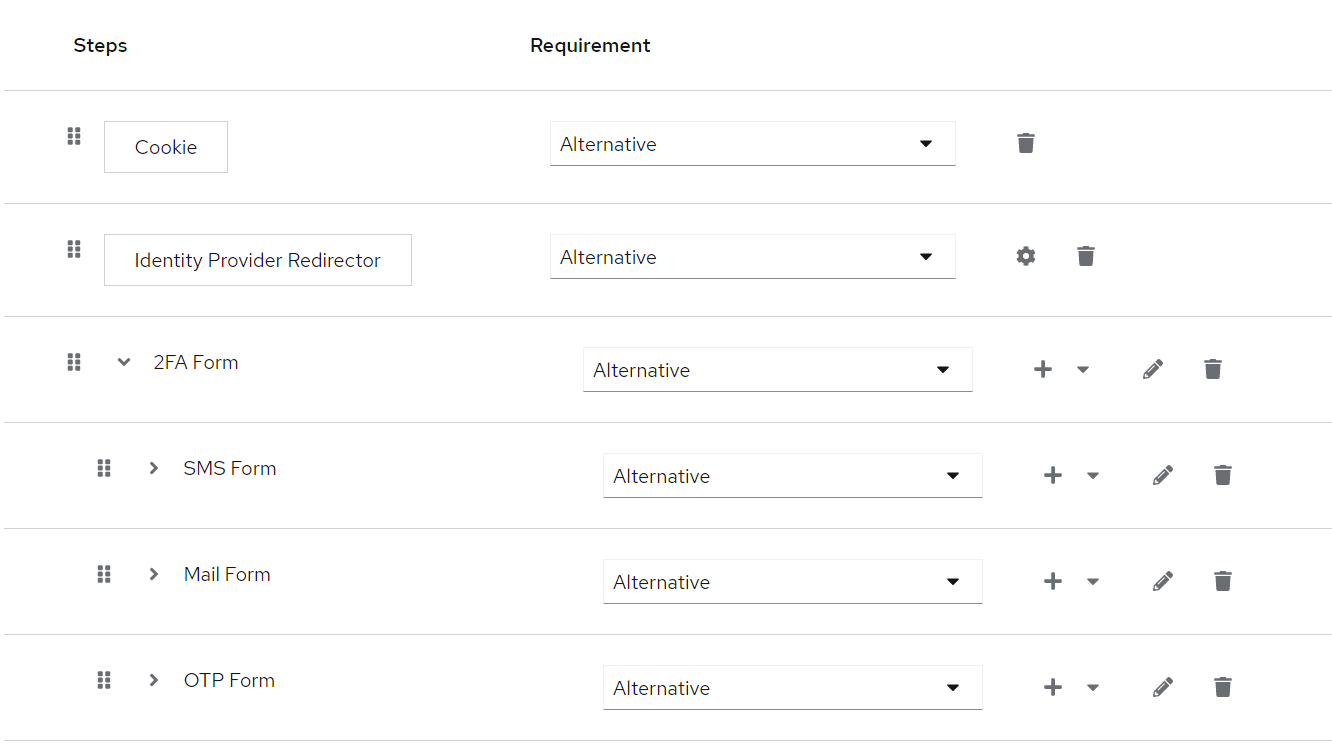
\includegraphics[width=\textwidth]{./img/Keycloak-AuthenticationFlow-BrowserFlow.png}
    \caption{Flow d'authentification du browser}
    \label{fig:keycloak_browser_2fa}
\end{figure}

Cet Authentication Flow possède 3 moyens de connexion : par Cookie, par Identity Provider et par le
formulaire 2FA. Si l'utilisateur utilise l'un de ses moyens, il sera authentifié et redirigé vers l'ACS.

Pour le formulaire 2FA, nous avons le choix entre 3 formulaires : SMS, Mail et OTP. Ces trois
formulaires ont le même fonctionnement. Ils contiennent chacun un formulaire Username \& Password, ainsi qu'un formulaire utilisé par le moyen 2FA. Ces deux formulaires sont obligatoires et sont donc en « Required ».

\begin{figure}[H]
    \centering
    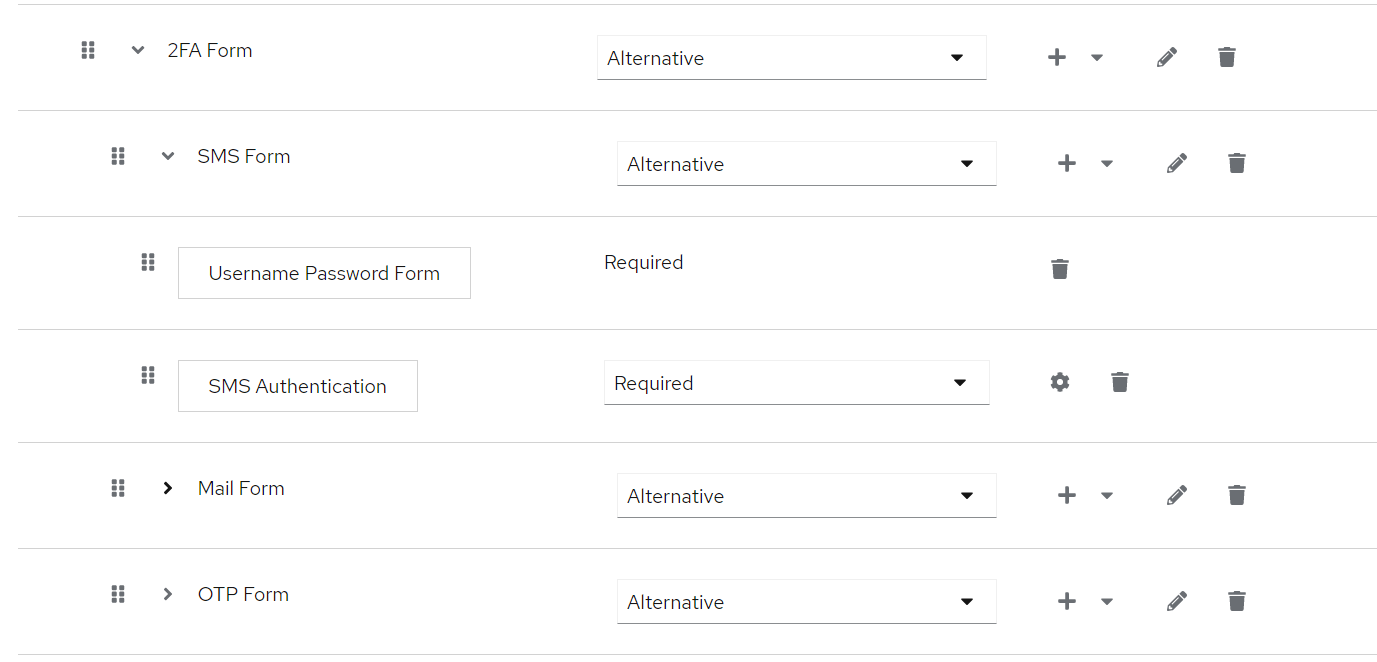
\includegraphics[width=\textwidth]{./img/Keycloak-AuthenticationFlow-2FAForm.png}
    \caption{Flow d'authentification 2FA}
    \label{fig:keycloak_flow_2fa}
\end{figure}

Les formulaires d'authentification via Mail et SMS sont gérés par des librairies externes que nous
détaillons au point suivant.

\subsubsection{Providers externes}

Keycloak supporte l'ajout de librairies externes. Nous en avons utilisé et créé pour:

\begin{itemize}
    \item La connexion 2FA via SMS
    \item La connexion 2FA via Mail
    \item La sauvegarde d'event customisée pour stockage sur une BD MongoDB
\end{itemize}

Pour ce faire, nous devons juste inclure le(s) fichier(s) .jar dans l'onglet provider du serveur de
Keycloak.

Pour la création de formulaire SMS et Mail, il faut obligatoirement créer deux classes : une qui
implémente l'interface Authenticator et une autre qui implémente l'interface AuthenticatorFactory.
Ces classes sont fournies dans la librairie open-source de Keycloak. La classe Authenticator va quand
à elle récupérer un fichier .ftl qui sera notre formulaire personnalisé. La classe AuthenticatorFactory
quant à elle va contenir toutes les informations du moyen d'authentification.

Pour l'enregistrement des events, nous avons créer une librairie contenant deux classes : une qui
implémente la classe EventListenerProvider et une autre qui implémente l'interface
EventListenerProviderFactory. Ces classes sont aussi fournis dans la librairie de Keycloak. La classe
EventListenerProvider va contenir la fonction onEvent, qui indiquera à l'application le comportement
à avoir selon l'évènnement reçu en paramètre. La classe EventListenerProviderFactory va contenir les
options lors de l'initialisation et la fermeture du listener, ainsi que les informations du provider dans
l'application Keycloak.
